\documentclass[main_estudante.tex]{subfiles}

\begin{document}

\chapter{Trigonometria e vetores}

\section{Questões diagnósticas}

\begin{diagnostico}
Considerando a figura ao lado, calcule:
\begin{enumerate}[a)]
  \item A medida do segmento $\overline{AB}$.
  \item Seja $D$ a outra extremidade da altura do triângulo relativa ao vértice $C$, calcule o comprimento de $\overline{BD}$.
\end{enumerate}
\end{diagnostico}
  
\begin{diagnostico}
Qual é a medida em graus do ângulo formado entre o eixo $X$ e o segmento de reta que liga a origem ao ponto $(3;1)$? \textit{Você pode usar a calculadora se julgar necessário.}
\end{diagnostico}

\section{Gabarito}

\textbf{Questão 1:} a) $3\sqrt{3}$, b) $9/2$. \textbf{Questão 2:} a) aproximadamente $18,4\degree$.

\section{Quadro de orientação}

\begin{center}
 \begin{tabular}{|c c c |c|} 
 \hline
 1A e 1B & 2 & Onde começar\\
 \hline
 C & E & Questão 2 \\ 
 \hline
 C & C & Questão 5 \\ 
 \hline
\end{tabular}
\end{center}

\section{Comentários iniciais}

Neste capítulo, serão trabalhados conteúdos relacionados a trigonometria e vetores. A intenção é focar em aspectos da trigonometria que estejam mais próximos do que será usado em Geometria Analítica, porém, limitados ao contexto do plano cartesiano (duas dimensões).

As questões propostas não serão arranjos complicados de segmentos e círculos nos quais propriedades geométricas devem ser identificadas. No geral, a interpretação geométrica das questões será simples e a atenção será focada no uso que se faz das relações seno e cosseno e na interpretação vetorial dessas relações.

Vetores serão utilizados na formulação de algumas questões ao invés de pontos e segmentos, que são mais comuns ao longo do Ensino Médio. A intenção é familiarizar o estudante com esse conceito sem explorar suas propriedades específicas.

As funções inversas, arcosseno e arcocosseno, também serão utilizadas com bastante frequência, mas a ênfase não será no comportamento delas como função, mas no seu uso para resolução e interretação de problemas de geometria plana.

Este capítulo difere dos demais deste material em uma outra característica. Livros de Geometria Analítica raramente lidam com objetos bidimensionais pois nesse contexto as generalizações por trás de conceitos como produto escalar e vetorial são pouquíssimo úteis (e relações trigonométricas bastam). Por isso, não foi possivel indicar referências externas ao longo do capítulo e usar uma questão de fato extraída de um livro-texto ao final. Enquanto isso certamente representa uma perda em termos da proposta do material , esperamos construir ao longo dele um entendimento conceitual mais robusto em duas dimensões de conceitos que serão estudados exaustivamente em mais dimensões em Geometria Analítica e Álgebra Linear.

\section{Questões comentadas}

\begin{questao}
Sabendo que $\overline{AB}=6$ na figura abaixo, calcule o comprimento dos segmentos:
\begin{enumerate}[a)]
\item $\overline{BC}$
\item $\overline{BD}$
\item $\overline{AD}$
\end{enumerate}
\end{questao}

\begin{figure}[h]
\centering
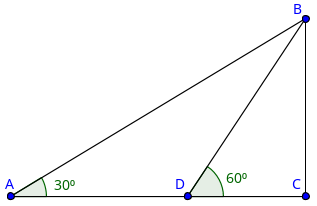
\includegraphics[width=0.4\textwidth]{./img/c4q1.png}
\end{figure}

O objetivo desta questão é iniciar o uso das relações trigonométricas seno e cosseno em um problema relativamente simples de geometria plana. O terceiro item é o único que não pode ser resolvido diretamente via aplicação de uma relação trigonométrica, ele exige o cálculo de $AC$ e $DC$. Além disso, a repsosta final depende de alguns cálculos envolvendo frações.

Se você achar que os estudantes tiveram dificuldade nessa questão proponha variações em torno da mesma configuração dando como valores iniciais os dois ângulos (note que o mais externo deve ser menor do que o interno e por enquanto é deseja usar apenas gulos notáveis) e o comprimento de um dos vários segmentos disponíveis. Como o objetivo é reforçar as relações trigonométricas e não praticar problemas de geometria, a repetição da configuração não é um problema.

\begin{questao}
Use o seu celular pra obter:
\begin{enumerate}[a)]
\item $\sin(\frac{4\pi}{9})$, arredondado para 2 casas decimais.
\item $\cos(\frac{\pi}{12})$, arredondado para 2 casas decimais.
\item $\sin(18\degree)$, arredondado para 1 casa decimal.
\item $\cos(22.5\degree)$, arredondado para 1 casa decimal.
\item $\cos(1,5)$, arredondado para 2 casas decimais.
\end{enumerate}
\end{questao}

A intenção dessa questão é apenas ter certeza de que os estudantes sabem usar a calculadora dos seus celulares para obter o seno e o cosseno de ângulos dados em graus e em radianos. Além disso, insista que façam os arredondamentos corretamente pois isso será usado ao longo deste capítulo todo.

O último item é intencionalmente dúbio: a falta do $\pi$ induz a leitura do valor sendo em graus, mas note que o símbolo \degree não está presente, portanto, trata-se sim de uma medida em radianos. A resposta obtida em cada caso é bastante diferente (o correto é um valor próximo de 0 pois $1,5$ é um pouco menor que $\pi/2$, ou seja, $90\degree$.

\begin{questao}
Sabendo que na figura abaixo $\overline{AC}=4$ obtenha a medida dos segmentos pedidos abaixo. Use uma calculadora se necessário.
\begin{enumerate}[a)]
\item A altura do triângulo relativa ao lado $\overline{AB}$.
\item $\overline{CB}$
\end{enumerate}
\end{questao}

\begin{figure}[h]
\centering
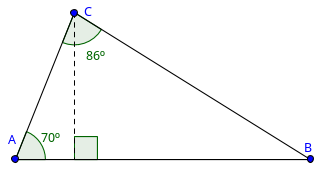
\includegraphics[width=0.5\textwidth]{./img/c4q3.png}
\end{figure}

A estrutura geométrica da questão não deve ser o foco da atenção dos estudantes, pois o objetivo desta questão é que usem a calculadora para obter o seno e cosseno de ângulos não notáveis. Propriedades básicas como a soma dos ângulos internos de um triângulo e o fato de o ângulo $\hat{C}$ não ser dividido ao meio pela altura podem emergir.

Assim como na primeira questão, você pode gerar variações dessa questão de maneira rápida: mesmo diagrama, dois ângulos dados e uma medida. 

\begin{questao}
Use as funções $\sin^{-1}$ e $\cos^{-1}$ da sua calculadora para obter:
\begin{enumerate}[a)]
\item A medida em radianos, com duas casas decimais, do ângulo cujo seno é igual a $0,7$. Procure pela opção DEG e RAD na calculadora para alternar entre graus e radianos.
\item A medida em radianos, com duas casas decimais, do ângulo cujo cosseno é igual a $0,4$.
\item A medida em graus, com zero casas decimais, do ângulo cujo seno é igual a $0,6$. 
\item A medida em graus, com zero casas decimais, do ângulo cujo cosseno é igual a $0,87$.
\end{enumerate}
\end{questao}

As funções arcosseno e arcocosseno são introduzidas aqui com o intuito de expandir as possibilidades de trabalho com ângulos e relações trigonométricas para além dos valores notáveis.

\begin{questao}
Considerando a imagem ao lado, calcule:
\begin{enumerate}[a)]
\item O comprimento do segmento $\overline{OP}$. \textit{$O$ se refere à origem, ou seja, ao ponto $(0;0)$}.
\item O seno e o cosseno do ângulo determinado pelo segmento $\overline{OP}$ e o eixo $X$. 
\item A medida em radianos e em graus desse ângulo.
\end{enumerate}
\end{questao}

\begin{figure}[h]
\centering
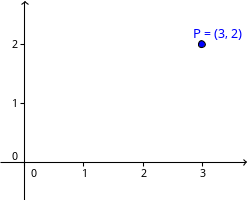
\includegraphics[width=0.5\textwidth]{./img/c4q5.png}
\end{figure}

\begin{questao}
Considere os dois vetores representados abaixo.
\begin{enumerate}[a)]
\item Calcule a norma de $\overrightarrow{V}$ e $\overrightarrow{U}$.
\item Obtenha, em graus, os ângulos determinados por $\overrightarrow{V}$ e $\overrightarrow{U}$.
\item Determine, em graus, a medida do ângulo entre $\overrightarrow{V}$ e $\overrightarrow{U}$.
\end{enumerate}
\end{questao}

\begin{figure}[h]
\centering
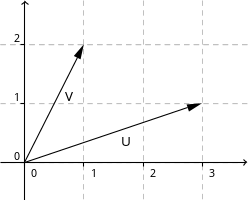
\includegraphics[width=0.5\textwidth]{./img/c4q6.png}
\end{figure}

Essas duas questões servem como fixação do uso das funções arcosseno e arcocosseno bem como para introduzir o eixo cartesiano e o conceito de vetor. Não se preocupe com tecnalidades do conceito de vetor neste ponto (isso é conteúdo para Geometria Analítica).

\begin{questao}
Determine as coordenadas e represente em um eixo cartesiano os vetores cuja norma e ângulo são dados abaixo.
\begin{enumerate}[a)]
\item Vetor $\overrightarrow{V}$ com norma $3$ e ângulo $40\degree$.
\item Vetor $\overrightarrow{U}$ com norma $2$ e ângulo $150\degree$.
\end{enumerate}
\end{questao}

Faça questão que os estudantes comecem a resolver essa questão fazendo um esboço destes vetores. A posição precisa não é importante, mas aproximações coerentes com os ângulos (o segundo vetor deve estar no segundo quadrante) e normas (o primeiro deve ser mais longo que o segundo) dadas são.

Para o segundo item, não use o valor de seno e cosseno de 150\degree, mas sim o fato de o vetor formar um ângulo de 30\degree com o lado negativo do eixo $X$. Além disso, nesse item deve-se utilizar o valor tabelado para o cosseno e seno de 30\degree e não a calculadora.

\begin{questao}
Considere os dois vetores dados ao lado. Vamos calcular a área do triângulo determinado pela origem e pela extremidade dos vetores sabendo que o ângulo entre eles é igual a $60\degree$, a norma de $\overrightarrow{A}$ é igual a $3$ e a de $\overrightarrow{B}$ igual a $5$.
\begin{enumerate}[a)]
\item Obtenha a norma dos vetores $\overrightarrow{A}$ e $\overrightarrow{B}$.
\item Obtenha a medida em graus dos ângulos determinados pelos vetores $\overrightarrow{A}$ e $\overrightarrow{B}$ e do ângulo entre eles.
\item Trace a altura do triângulo relativa à $\overrightarrow{B}$.
\item Calcule o comprimento dessa altura usando o seno do ângulo entre os vetores.
\item Calcule a área do triângulo usando $\overrightarrow{B}$ como base.
\end{enumerate}
\end{questao}

\begin{figure}[h]
\centering
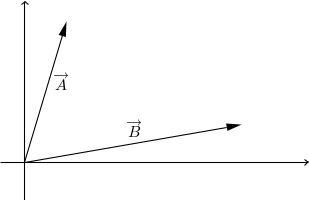
\includegraphics[width=0.6\textwidth]{./img/c4q8.png}
\end{figure}

\begin{questao}
Calcule a área do triângulo determinado pelos vetores $\overrightarrow{V}=(2;2)$ e $\overrightarrow{U}=(4;1)$ usando o metodo descrito acima.
\end{questao}

Essas duas questões tem o objetivo de mostrar a relação entre o seno e a área compreendida entre dois vetores. O mesmo raciocínio poderia ser aplicado ao paralelogramo determinado pelos dois vetores. Essa relação é central para a definição do produto vetorial. A grande diferença é que o produto vetorial generaliza essa relação para contextos com mais dimensões e foco nas coordenadas dos vetores, como seria de se esperar em geometria analítica.

Vale ressaltar que o ângulo entre os vetores também poderia ser calculado com auxílio de fórmulas para obter $\sin(a-b)$ e $\cos(a-b)$, mas esse não é o nosso foco já esse recurso é pouco utilizado em Geometria Analítica, onde as coordenadas dos vetores são utilizadas com mais frequência do que conceitos de geometria plana.

\begin{questao}
Considere os dois vetores dados ao lado. Vamos calcular a área do triângulo determinado pela origem e pela extremidade dos vetores sabendo que o ângulo entre eles é igual a $60\degree$, a norma de $\overrightarrow{A}$ é igual a $3$ e a de $\overrightarrow{B}$ igual a $5$.
\begin{enumerate}[a)]
\item Obtenha a norma dos vetores $\overrightarrow{A}$ e $\overrightarrow{B}$.
\item Obtenha a medida em graus dos ângulos determinados por $\overrightarrow{A}$ e $\overrightarrow{B}$ e do ângulo entre eles.
\item Trace a altura relativa à $\overrightarrow{B}$ e chame de $C$ a intersecção dessa altura com $\overrightarrow{B}$.
\item Calcule o comprimento do vetor $\overrightarrow{OC}$.
\end{enumerate}
\end{questao}

\begin{reflita}
 Descreve com suas palavras como você deve proceder para obter o comprimento da projeção ortogonal de um vetor dado sobre um segundo vetor dado.
\end{reflita}

\begin{questao}
\item Calcule o comprimento da projeção ortogonal de $\overrightarrow{V}=(1;\sqrt{3})$ em $\overrightarrow{U}=(2;2)$.
\end{questao}

Dessa vez, o objetivo é explorar a relação entre cosseno e produto escalar. Lembre-se que o produto escalar entre dois vetores é nulo quando estes são ortogonais e é máximo quando os vetores são múltiplos um do outro (ângulo entre eles igual a 0), exatamente o mesmo que ocorre com o cosseno.

Na terceira questão, os vetores dados determinam ângulos notáveis. Por terem vindo de uma sequência de questões que foram resolvidas com auxílio da calculadora, os estudantes talvez não notem esse fato, mas vale a pena salientar, não como algo imprescindível mas sim como uma propriedade que potencialmente facilita a resolução da questão.

\begin{questao}
Considere o vetor $\overrightarrow{V}=(4;3)$.
\begin{enumerate}[a)]
\item Qual é a norma deste vetor?
\item Divida as duas dimensões de $\overrightarrow{V}$ pela sua norma de modo a obter um novo vetor que chamaremos de $\overrightarrow{V_1}$. Qual é a norma de $\overrightarrow{V_1}$?
\item Se você dobrar as dimensões de $\overrightarrow{V_1}$ o que vai ocorrer com a sua norma?
\end{enumerate}
\end{questao}

Essa questão introduz a ideia de obter múltiplos, unitários ou não, de um vetor dado. Ela é uma preparação para decomposição de vetores, que será o conceito central da seção Rumo ao livro-texto.

\section{Rumo ao livro texto}

A proposta desta questão é reunir o que foi feito com seno, cosseno e norma nas questões anteriores para entender como decompor um vetor dado em dois vetores perpendiculares. Espera-se que ao compreender o processo no caso bidimensional, os estudantes tenham condição de compreender melhor tanto esse processo quanto alguns outros similares em Geometria Analítica.

\begin{resolvida}
Decomponha o vetor $\overrightarrow{V}=(1;3)$ como soma de dois vetores perpendiculares de modo que um deles esteja na mesma direção do vetor $\overrightarrow{A}=(1;1)$.
\end{resolvida}

A resolução está descrita detalhadamente no caderno do estudantes. Insista que leiam com atenção antes de tentar resolver a questão proposta.

\begin{resolva}
Decomponha o vetor $\overrightarrow{V}=(3;4)$ como soma de dois vetores perpendiculares de modo que um deles esteja na mesma direção do vetor $\overrightarrow{A}=(12;5)$.
\end{resolva}

Os dois vetores que respondem a esta questão são $\overrightarrow{V_A}=(4,0;1,7)$ e $\overrightarrow{V_B}=(-1,0;2,3)$. Insista que os estudantes representem os vetores ao longo da resolução para que entendam as etapas da resolução e os conceitos envolvidos.

\section{Gabarito}

\noindent\textbf{Questão 1:} a) $3$, b) $3\sqrt{3}/2$, c) $9\sqrt{3}/4$.

\noindent\textbf{Questão 2:} a) $0,98$, b) $0,26$, c) $0,3$, d)$0,9$, e) $0,07$.

\noindent\textbf{Questão 3:} a) $3,76$, b) $9,24$.

\noindent\textbf{Questão 4:} a) $0,78$, b) $1,16$, c) $37\degree$, d) $30\degree$.

\noindent\textbf{Questão 5:} a) $\sqrt{13}$, b) $2\sqrt{13}/13$ e $3\sqrt{13}/13$, c) $0,59$ e $34\degree$.

\noindent\textbf{Questão 6:} a) $\Arrowvert V \Arrowvert = \sqrt{5}$ e $\Arrowvert U \Arrowvert = \sqrt{10}$, b) $63\degree$ e $18\degree$, c) $45\degree$.

\noindent\textbf{Questão 7:} a) $(2,30;1,93)$, b) $(\sqrt{3};1,00)$.

\noindent\textbf{Questão 8:} c) $\sqrt{10}/2$, d) $\frac{5}{2}$.

\noindent\textbf{Questão 9:} a) $2,42$.

\noindent\textbf{Questão 10:} a) $2.301$, b) $1.301$, c) $0.301$.

\noindent\textbf{Questão 11:} $1,93$.

\noindent\textbf{Questão 12:} a) $5$, b) $1$, c) dobrar também.

\section{Questões adicionais}

\begin{adicional}
Decomponha o vetor $\overrightarrow{V}=(2;2\sqrt{3})$ em uma soma de vetores perpendiculares de modo que um deles esteja na direção sugerida pelo vetor $\overrightarrow{A}=(4;-2)$.
\end{adicional}

Essa questão é similar ao que foi discutido na seção Rumo ao Livro-texto, mas usa pela primeira vez um vetor que não está no primeiro quadrante. Isso foi usado com reserva ao longo deste capítulo porque não estamos trabalhando com ângulos maiores do que 90\degree por enquanto. Entretanto, essa questão pode ser resolvida sem que isso seja necessário, basta observar o comportamento dos ângulos após representar os vetores no plano cartesiano.

\begin{adicional}
Considere os vetores $\overrightarrow{A}=(\sqrt{3};1)$ e $\overrightarrow{B}=(-1;1)$.
\begin{enumerate}[a)]
\item Esboce com cuidado ambos em um plano cartesiano.
\item Esboce a decomposição de $\overrightarrow{B}$ como uma soma de vetores perpendiculares de modo que um deles esteja na direção sugerida pelo vetor $\overrightarrow{A}$
\item Estime visualmente as coordenadas da decomposição de $\overrightarrow{B}$.
\end{enumerate}
\end{adicional}

O objetivo dessa questão é que os estudantes discutam como deve se comportar a decomposição de vetores cujo ângulo de separação seja maior do que 90\degree. O cálculo em si não é importante, pois o procedimento já foi repetido pelos estudantes algumas vezes ao longo do capítulo, por isso incentive: o cuidado com o esboço do item a e a discussão em torno do item b.

Como este capítulo foi totalente baseado em vetores com apenas duas dimensões, não foi possível indicar materiais complementares. Caso algum estudante chegue a este ponto antes do final das atividades, sugerimos a leitura da seção 8.1 do livro \sugestao{Álgebra Linear} para uma introdução ao produto escalar e vetorial ou da seção 3.1 do livro \sugestao{Matrizes, Vetores e Geometria Analítica} sobre soma, subtração e multiplicação por escalas de vetores.

\end{document}
